\documentclass[a4paper,12pt]{article}
\usepackage[english,ukrainian,russian]{babel}
\linespread{1}
\usepackage{ucs}
\usepackage[utf8]{inputenc}
\usepackage[T2A]{fontenc}
\usepackage[paper=portrait,pagesize]{typearea}
\usepackage{amsmath}
\usepackage{bigints}
\usepackage{amsfonts}
\usepackage{graphicx}
\usepackage{amssymb}
\usepackage{cancel}
\usepackage{gensymb}
\usepackage{multirow}
\usepackage{rotate} 
\usepackage{pdflscape}
\usepackage{bigstrut}
\usepackage[pageanchor]{hyperref}
\usepackage{chngpage}
\usepackage{fancybox,fancyhdr}
\newcommand\tab[1][1cm]{\hspace*{#1}}
\newcommand{\arch}{\textrm{arcch}}
\newcommand{\arsh}{\textrm{arcsh}}
\newcommand{\dint}{\displaystyle\int}
\newcommand{\dsum}{\displaystyle\sum}
\newcommand{\RomanNumeralCaps}[1]{\MakeUppercase{\romannumeral #1}}
\usepackage[left=15mm, top=20mm, right=15mm, bottom=15mm, nofoot]{geometry}

\usepackage{listings}
\usepackage{xcolor}
\definecolor{codegreen}{rgb}{0,0.6,0}
\definecolor{codegray}{rgb}{0.5,0.5,0.5}
\definecolor{codepurple}{rgb}{0.58,0,0.82}
\definecolor{backcolour}{rgb}{0.95,0.95,0.92}
\definecolor{keywordcolor}{rgb}{0.0, 0.5, 0.9}

\lstdefinestyle{pythonstyle}{
    backgroundcolor=\color{backcolour},   
    commentstyle=\color{codegreen}\itshape,
    keywordstyle=\color{keywordcolor}\bfseries,
    numberstyle=\tiny\color{codegray},
    stringstyle=\color{codepurple},
    basicstyle=\ttfamily\footnotesize,
    breakatwhitespace=false,         
    breaklines=true,                 
    captionpos=b,                    
    keepspaces=true,                 
    numbers=left,                    
    numbersep=5pt,                  
    showspaces=false,                
    showstringspaces=false,
    showtabs=false,                  
    tabsize=4,
    frame=shadowbox,
    language=Python,
    morekeywords={self, as, None, True, False, with, yield}
}
\lstset{style=pythonstyle}

\begin{document}
    \pagestyle{fancy}
    \fancyhead{}
    \fancyhead[R]{ФІ-12 Завалій Олександр}
    \begin{center}
        \large{\textbf{Міністерство освіти і науки України\\
                Національний технічний університет України\\
                «Київський політехнічний інститут імені Ігоря Сікорського»\\
                Навчально-науковий Фізико-технічний інститут}}\\
        \hfill \break \hfill \break \hfill\break \hfill \break \hfill \break \hfill \break \hfill \break
        \hfill \break \hfill \break \hfill \break
        \begin{center}
            \normalsize{\textbf{Моделювання природничих, \\ економічних та соціальних процесів\\
            Практичне завдання №1}}
        \end{center}
    \end{center}
    \hfill \break \hfill \break \hfill \break \hfill \break \hfill \break \hfill \break \hfill \break
    \hfill \break \hfill \break \hfill \break \hfill \break 
    \begin{flushright}
        \large{ \hspace{35pt} Виконав:\\
            студент групи ФI-12\\
            Завалій Олександр\\} 
        %\large{ \hspace{35pt} Перевірив:\\
        %} 
    \end{flushright}
    \hfill \break \hfill \break 
    \hfill \break \hfill \break \hfill \break \hfill \break \hfill \break \hfill \break \hfill \break
    \hfill \break
    \begin{center} \textbf{Київ-2025} \end{center}
    \thispagestyle{empty}

\newpage
    \begin{center}
        \section*{\bfseries{Практичне завдання №1. \\
        Використання математичних моделей для покращення бізнес-стратегій у готельній та ресторанній індустрії. Наслідки для економічної стабільності.
        }}
    \end{center}
    \noindent
    Зміст індивідуального завдання:
    \begin{enumerate}
        \item Підготуйте звіт (1-2 сторінки), відповівши на наступні питання:
        \begin{enumerate}
            \item Постановка задачі: Яку бізнес‑проблему вирішувала модель?
            \item Математичні підходи: Які методи та моделі були застосовані? (коротко, з посиланням на ключові поняття лекції)
            \item Висновки: Які загальні висновки можна зробити про ефективність застосування математичного моделювання у цьому випадку?
        \end{enumerate}
        \item Додаткове завдання 1 (на +1 бал) \\
        Дати відповіді на наступні питання:
        \begin{enumerate}
            \item Практичне значення: Які результати були отримані і як вони вплинули на бізнес‑рішення? (за наявності – зазначте економічний ефект)
            \item Обмеження моделі: Які потенційні обмеження має модель і які чинники можуть вплинути на точність прогнозів?
        \end{enumerate}
        \item Додаткове завдання 2 (на +2 бали) \\
        Реалізуйте моделювання обраного кейсу або статті у вигляді Python‑скрипту з використанням бібліотек, таких як NumPy, SciPy та Matplotlib (або інше). Код має бути коментованим та/або містити короткий опис основних етапів моделювання.
    \end{enumerate}

\newpage
    \begin{center}
        \Large{Task \RomanNumeralCaps{1}}
    \end{center}
    \textbf{Постановка задачі:} \\
    В статті розглянуто проблему оптимізації процесів прийняття рішень у готельній та ресторанній індустрії для сприяння 
    економічній стабільності за допомгою математичних моделей.  
    Дослідження визначає ключові фактори, що впливають на ефективність бізнесу. Серед розглянутих факторів можемо відзначити задоволеність 
    клієнтів, стратегії ціноутворення та розподіл ресурсів. Отже основна мета полягає у розробці математичних моделей для підтримки рішень на основі вхідних даних. \\
    \textbf{Математичні підходи:} \\
    У дослідженні використовувалися три основні математичні підходи:
    \begin{enumerate}
        \item Регресійний аналіз. \\
        Множинна регресія використовувалася для кількісного визначення взаємозв’язків між незалежними змінними 
        (стратегіями ціноутворення, маркетинговими витратами) і залежними змінними (задоволеністю клієнтів, доходом).
        Цей метод можемо віднести до аналітичної моделі, адже ми маємо точний розв'язок у вигляді формули.
        \item Аналіз часових рядів(ARIMA). \\
        Моделі ARIMA були застосовані для прогнозування рівня заповнюваності, це допоможе краще зрозуміти сезонні тенденції.
        Ця модель відноситься до моделей за часовою дискретизацією, тобто дискретна модель.
        \item Моделі оптимізації. \\ 
        Методи лінійного програмування були застосовані для оптимізації планування робочої сили та управління запасами, 
        щоб максимізувати дохід при дотриманні операційних обмежень.
        Я думаю, що цю модель можемо віднести до аналітичної, адже вона надає точне математичне рішення.
    \end{enumerate}
    \textbf{Висновки:} \\
    У цьому дослідженні можемо відзначити сильні сторони у використанні математичних моделей задля підвищенні ефективності прийняття рішень й операцій. 
    Регресійна модель підкреслила важливість цінових та маркетингових стратегій. Вона показала, що визначені фактори пояснюють 
    приблизно 65\% відхилень у доходах, підкріплюючи гіпотезу про те, що стратегічне ціноутворення та цілеспрямовані 
    маркетингові зусилля є важливими для максимізації доходів.
    Модель ARIMA відображає типові коливання попиту, що характерні для цієх індустрії. Це підтверджує необхідність компаній адаптувати 
    свої стратегії на основі прогнозування. Здатність точно прогнозувати попит життєво важлива для ефективного розподілу ресурсів і ефективності роботи.
    Лінійне програмування надає можливість оптимізувати розподіл ресурсів. Цей висновок вказує на важливість збалансування витрат на оплату праці 
    та управління запасами, підкріплюючи аргумент, що математичне моделювання може підвищити операційну ефективність і прибутковість. 
    Загалом, інтеграція цих моделей у бізнес-стратегії сприяє економічній стабільності та стійкості.

\newpage
    \begin{center}
        \Large{Task \RomanNumeralCaps{2}}
    \end{center}
    \textbf{Практичне значення:} \\
    Результати дослідження продемонстрували, як підходи на основі даних моделей можуть підвищити прибутковість. Можемо відзначити ключові результати:
    \begin{enumerate}
        \item Прогнозоване збільшення доходу на 5\% завдяки оптимізованій стратегії ціноутворення.
        \item Підвищення ефективності робочої сили завдяки оптимізованому плануванню.
        \item Зниження витрат на запаси завдяки підтримці оптимального рівня запасів.
    \end{enumerate}
    Економічний ефект від застосування моделей відображає підвищення прибутковості та зниженні експлуатаційних витрат. \\
    \textbf{Обмеження моделі:}
    \begin{enumerate}
        \item Прогнози часових рядів можуть бути неточними, якщо майбутні умови значно відрізняються від минулих тенденцій.
        \item Моделі лінійного програмування можуть занадто спрощувати реальні обмеження.
        \item Економічні події, нормативні зміни або стихійні лиха можуть вплинути на точність моделі.
    \end{enumerate}
    Майбутні вдосконалення можуть передбачати інтеграцію методів машинного навчання для більш адаптивного прогнозування та розширення моделей 
    оптимізації з додатковими обмеженнями.

\newpage
    \begin{center}
        \Large{Task \RomanNumeralCaps{3}}
    \end{center}
    \begin{lstlisting}[language=Python]
import os
import matplotlib.pyplot as plt
from scipy.optimize import linprog
from statsmodels.tsa.arima.model import ARIMA
path = os.getcwd().replace('Model', 'Results')

# 2. Time Series Analysis (Occupancy Forecasting)
occupancy_data = [78, 80, 75, 70, 65, 72]  # Input data on occupancy
model = ARIMA(occupancy_data, order=(1,1,1))  # Create ARIMA model with parameters (p=1, d=1, q=1)
fit = model.fit()  # Train the model on the input data
forecast = fit.forecast(steps=6)  # Forecast for the next 6 months

# Visualization of input data and forecast
plt.plot(range(1,7), occupancy_data, label='Historical')  # Input data
plt.plot(range(7,13), forecast, label='Forecast', linestyle='--')  # Forecast
plt.xlabel('Month')
plt.ylabel('Occupancy Rate (%)')
plt.title('Occupancy Rate Forecast')
plt.legend()
plt.grid(True)
plt.savefig(f'{path}/Occupancy Rate Forecast.jpg')
plt.show()
    \end{lstlisting}
    \begin{minipage}[h]{1\linewidth}
        \centering
        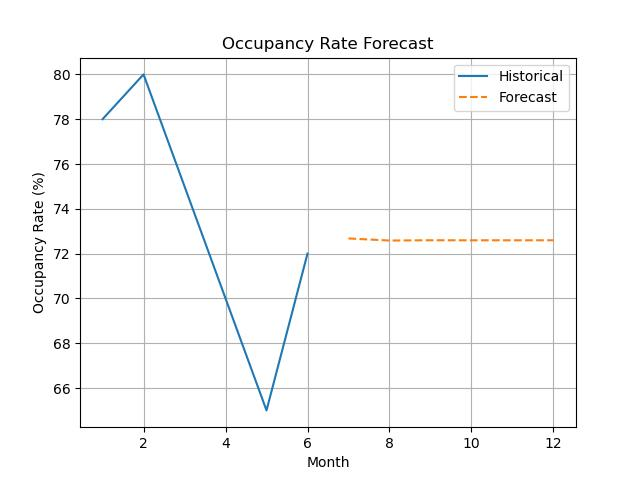
\includegraphics[width=0.9\linewidth]{Results/Occupancy Rate Forecast.jpg}  
    \end{minipage}

\newpage
    \begin{lstlisting}[language=Python]
# 3. Optimization Model (Maximizing Revenue with Constraints on Personnel and Inventory)
c = [-50, -20]  # Coefficients for revenue from each worker and unit of inventory (negative for maximization)
A = [[1, 0], [0, 1]]  # Constraints on personnel and inventory (one constraint per variable)
b = [30, 500]  # Maximum allowed number of personnel and inventory
result = linprog(c, A_ub=A, b_ub=b, method='highs')  # Solve linear optimization

# Output optimal personnel and inventory distribution
print(f'Optimal Staffing: {result.x[0]}, Optimal Inventory: {result.x[1]}')

Output:
Optimal Staffing: 30.0, Optimal Inventory: 500.0
    \end{lstlisting}

\newpage
\noindent
    \textbf{References:} 
    \begin{enumerate}
        \item[[1]] Kruhlyanko A., Peniuk V., Ursakii Y., Verstiak O. (2025 January) 
        Mathematical Modeling for Enhancing Business Strategies in the Hotel and Restaurant Industry: Implications for Economic 
        Stability \href{https://doi.org/10.52783/anvi.v28.3066}{(Click)}.
    \end{enumerate}

\end{document}